\section{Les 8 -- Elliptische krommen en lineaire codes}

\subsection*{Herhaling: discrete logaritmes in cyclische groepen}

We vertrekken van een \hl{cyclische groep} $G$ van eindige orde $n$, met een gekozen generator $g$. Dan kunnen alle elementen geschreven worden als:
\begin{equation*}
    G = \{e, g, g^2, \dots, g^{n-1}\}, \qquad g^n = e
\end{equation*}
Voor een element $h \in G$ bestaat er dan een unieke exponent
\begin{equation*}
    a \in \{0, 1, \dots, n-1\}
\end{equation*}
zodat
\begin{equation*}
    h = g^a
\end{equation*}
Deze exponent noemen we het \hl{discrete logaritme} van $h$ ten opzichte van $g$:
\begin{equation*}
    a = \log_g(h)
\end{equation*}
Het \hl{discrete-logaritmeprobleem} of \hl{DLP} is dan:
\begin{equation*}
    \text{Gegeven } g \text{ en } h = g^a \quad \to \quad \text{vind } a
\end{equation*}
Het cruciale verschil met gewone logaritmes is dat discrete logaritmes in goed gekozen groepen zeer moeilijk te berekenen zijn. Dit is de veiligheidsaanname achter veel publieke-sleutelcryptografie.

\subsubsection*{Generieke aanvallen en groepsgrootte}

Er bestaan generieke aanvallen die in elke groep werken. In de cursus wordt de methode aangehaald die gebaseerd is op \hl{Pohlig-Hellman-reductie}.

\begin{nicefact}*[Pohlig-Hellman-reductie]
    \nextpart[]*
    Het DLP is een groep van orde
    \begin{equation*}
        n = |G| = p_1^{e_1} p_2^{e_2} \cdots p_r^{e_r}
    \end{equation*}
    kan via \hl[factcolor!75!black]{Pohlig-Hellman} gereduceerd worden naar het berekenen van discrete-logaritmeproblemen in groepen van orde $p_i$.
\end{nicefact}

Gebaseerd op dit feit formuleerde \emph{Pollard} een algoritme dat werkt in alle groepen, genaamd \hl{Pollard's rho-methode}, dat een DLP in een groep van priemorde $p$ oplost in ongeveer $\sqrt{p}$ groepsoperaties.

$\rightwhitearrow$ Daarom nemen we in cryptografie meestal een groep van \hl{grote priemorde} $p$, want als de orde factoriseerbaar is, kan Pohlig-Hellman het probleem reduceren naar kleinere groepen.

Voor \hl{128-bit veiligheid} wil men dat een aanvaller ongeveer $2^{128}$ operaties nodig heeft. Omdat Pollard rho ongeveer $\sqrt{p}$ operaties vraagt, moet
\begin{equation*}
    \sqrt{p} \approx 2^{128}
\end{equation*}
dus $p \approx 2^{256}$. Daarom zijn groepen van ongeveer \hl{256 bits} voldoende als er geen betere aanval bekend is dan Pollard rho.

\subsubsection*{Twee belangrijke DLP-groepen}

\SimpleHeading{Multiplicatieve groep van een eindig veld}

Een historisch belangrijk voorbeeld is
\begin{equation*}
    \langle\mathbb{F}_q^\times, \cdot \rangle 
\end{equation*}
Dit is de eenhedengroep van een eindig veld, of een cyclische deelgroep daarvan.
Dit was het oorspronkelijke voorstel van \emph{Diffie} en \emph{Hellman}. Het probleem is echter dat voor deze groepen betere aanvallen bestaan dan Pollard rho, namelijk \hl{index-calculus-methoden}, waaronder de \hl{number field sieve}. \newline
$\rightwhitearrow$ Gevolg: voor 128-bit veiligheid heeft men een veldgrootte van ongeveer
\begin{equation*}
    q \approx 2^{3072}
\end{equation*}
nodig. Dit leidt tot veel grotere sleutels.

\SimpleHeading{Elliptische krommen over eindige velden}

Het belangrijkste moderne voorbeeld is een cyclische deelgroep van de groep van punten op een elliptische kromme over een eindig veld:
\begin{equation*}
    \langle E\left(\mathbb{F}_q, +\right) \rangle
\end{equation*}
Dit werd voorgesteld foor \emph{Koblitz} en \emph{Miller} in 1985. Voor elliptische krommen zijn geen index-calculus-aanvallen bekend die vergelijkbaar zijn met die voor $\mathbb{F}_q^\times$. Daarom is ongeveer
\begin{equation*}
    q \approx 2^{256}
\end{equation*}
voldoende voor 128-bit veiligheid.

Tegenvoorbeeld: in de groep $\langle \mathbb{F}_p, \textcolor{Red}{+}\rangle$ is DLP gemakkelijk. Dit wordt aangetoond in \cref{ex:l8_groep-DLP-easy}.

\subsubsection*{Protocols op basis van het DLP}

We gaan hier niet opnieuw dieper in op de protocollen, maar de volgende zijn gebaseerd op het DLP:
\begin{itemize}
    \item Diffie-Hellman-sleuteluitwisseling: gebruikt om een gedeelde geheime sleutel af te spreken. (\Cref{sec:l7_diffie-hellman})
    \item ElGamal-encryptie: een encryptie-systeem gebaseerd op DLP. (\Cref{sec:l7_elgamal})
    \item Schnorr-handtekeningen: een digitaal handtekeningsschema gebaseerd op DLP. (\Cref{sec:l7_schnorr})
\end{itemize}

\subsection{Elliptische krommen}

\SimpleHeading{Definitie}

We werken over een veld $K$ met karakteristiek niet gelijk aan 2 of 3:
\begin{equation*}
    \operatorname{char}(K) \neq 2, 3
\end{equation*}

\underbar{Herinner:} De \hl{karakteristiek} van een veld $K$ is simpelweg: hoe vaak moet je het getal 1 bij zichzelf optellen om op 0 uit te komen?
\begin{itemize}
    \item Gewone getallen ($\mathbb{R}$, $\mathbb{Q}$, $\mathbb{C}$): Als je $1 + 1 + 1 + \dots$ doet, kom je nooit op 0 uit. De karakteristiek is hier dus 0.
    \item Eindige velden ($\mathbb{F}_p$): Hier rekenen we modulo een priemgetal $p$. Bijvoorbeeld:
    \begin{itemize}
        \item In $\mathbb{F}_5$ geldt: $1 + 1 + 1 + 1 + 1 = 5 \equiv 0 \pmod 5$. De karakteristiek is hier 5.
        \item In $\mathbb{F}_2$ geldt: $1 + 1 = 2 \equiv 0 \pmod 2$. De karakteristiek is hier 2.
    \end{itemize}
\end{itemize}
Dus $\operatorname{char}(K) \neq 2,3$ wil zeggen: het veld waarin we werken mag géén modulo 2 or 3 rekenen zijn. En $K$ mag dus ook geen \textcolor{WildStrawberry}{uitbreidingsveld} hiervan zijn, zoals $\mathbb{F}_{2^m}$!

\begin{nicedefinition}*[Elliptische Kromme]
    \nextpart[]*
    Een \hl[PineGreen!75!black]{elliptische kromme} over een veld $K$ is dan een vlakke kromme van de vorm
    \begin{equation*}
        E : y^2 = x^3 + Ax + B
    \end{equation*}
    waarbij $A, B \in K$ en
    \begin{equation*}
        4A^3 + 27B^2 \neq 0
    \end{equation*}
    Deze laatste voorwaarde betekent dat de kromme \hl[PineGreen!75!black]{niet-singulier} is. Dat wil zeggen dat de kromme overal glas is, en dus geen scherpe punten of "zelf-doorsnijdingen" heeft. Algebraïsch heeft de derdegraadsvergelijking $x^3 + Ax + B = 0$ geen meervoudige wortels.

    \vspace{0.20cm}

    Voor ons is het vooral belangrijk dat de raaklijn in elk punt goed gedefinieerd is.
\end{nicedefinition}

\newpage
\SimpleHeading{Intuïtie over de vorm}

Over $\mathbb{R}$ kan je een elliptische kromme tekenen. Typisch zie je vormen zoals hieronder: één verbonden component of twee componenten.

\begin{center}
\resizebox{1.0\textwidth}{!}{%
    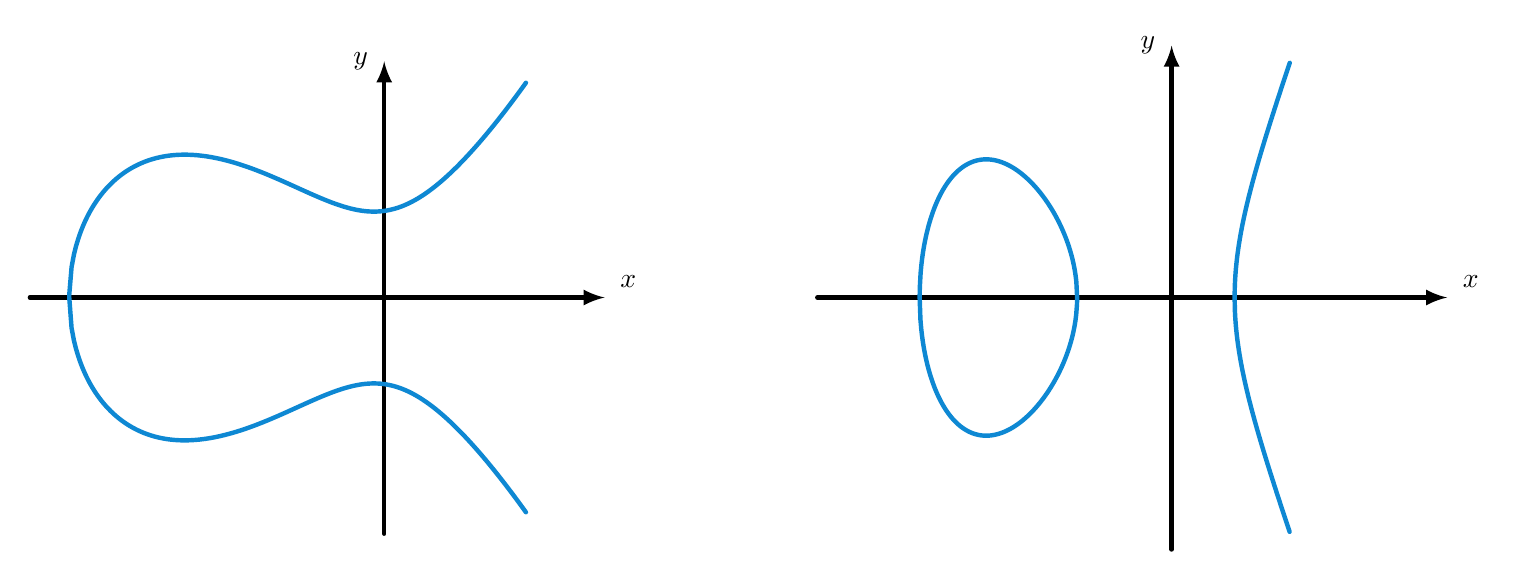
\begin{tikzpicture}[>=latex, line cap=round, line join=round]

% --- Global TikZ Styles for Consistency ---
\tikzset{
    axis/.style={
        ->,
        >=latex,
        ultra thick,
        draw=black
    },
    axisline/.style={
        ultra thick,
        draw=black
    },
    elliptic/.style={
        draw=cyan!70!blue,
        line width=1.6pt
    }
}

% =========================================================================
% --- Left Elliptic Curve: Vertically compressed ---
% =========================================================================
\begin{scope}[xshift=0cm]

    % --- Axes ---
    \draw[axisline] (-4.5,0) -- (1.8,0); % x-axis line
    \draw[axis] (1.8,0) -- (2.8,0);      % x-axis arrow

    \draw[axisline] (0,-3.0) -- (0,0);   % y-axis line
    \draw[axis] (0,0) -- (0,3.0);        % y-axis arrow

    \node at (3.1,0.2) {$x$};
    \node at (-0.3,3.0) {$y$};

    % --- Plotting with a 0.55 multiplier for a flatter look ---
    \draw[elliptic]
        plot[domain=1.80:-4, samples=200] (\x, {0.55 * sqrt(abs(\x*\x*\x + 4*\x*\x + \x + 4))})
        -- 
        plot[domain=-4:1.80, samples=200] (\x, {-0.55 * sqrt(abs(\x*\x*\x + 4*\x*\x + \x + 4))});

\end{scope}

% =========================================================================
% --- Right Elliptic Curve: Shifted left and bounded ---
% =========================================================================
\begin{scope}[xshift=10cm]

    % --- Axes ---
    \draw[axisline] (-4.5,0) -- (2.5,0); % x-axis line
    \draw[axis] (2.5,0) -- (3.5,0);      % x-axis arrow

    \draw[axisline] (0,-3.2) -- (0,0);   % y-axis line
    \draw[axis] (0,0) -- (0,3.2);        % y-axis arrow

    \node at (3.8,0.2) {$x$};
    \node at (-0.3,3.2) {$y$};

    % --- Closed Oval Component ---
    % Shifted left by 1.2 units (\x - 1.2) so it sits entirely to the left of the y-axis
    \draw[elliptic]
        plot[domain=0:-2, samples=200] (\x - 1.2, {sqrt(abs(\x*\x*\x - 4*\x))})
        -- 
        plot[domain=-2:0, samples=200] (\x - 1.2, {-sqrt(abs(\x*\x*\x - 4*\x))})
        -- cycle;

    % --- Right infinite component ---
    % Domain reduced from 3.5 to 2.7 to prevent overshooting the y-axis limits
    \draw[elliptic]
        plot[domain=2.7:2, samples=200] (\x - 1.2, {sqrt(abs(\x*\x*\x - 4*\x))})
        -- 
        plot[domain=2:2.7, samples=200] (\x - 1.2, {-sqrt(abs(\x*\x*\x - 4*\x))});

\end{scope}

\end{tikzpicture}
}
\end{center}

De vergelijking is symmetrisch in $y$, want als $(x,y)$ op de kromme ligt, dan ligt ook $(x, -y)$ op de kromme.

De snijpunten met de $x$-as vind je door $y=0$ te zetten:
\begin{equation*}
    x^3 + Ax + B = 0
\end{equation*}
Over $\mathbb{C}$ heeft deze derdegraadsvergelijking drie nulpunten. Over $\mathbb{R}$ zijn er ofwel één, ofwel drie reële nulpunten, omdat niet-reële nulpunten in complex toegevoegde paren voorkomen.

\SimpleHeading{Geen ellips}

Een elliptische kromme is \hl{geen ellips}. De naam komt gewoon historisch van de studie van de omtrek van een ellips, waarvij elliptische integralen optreden.

\subsubsection{Punten op een elliptische kromme}

De puntenverzameling noteren we als $E(K)$. Ze bestaat uit alle oplossingen $(a,b) \in K^2$ van
\begin{equation*}
    b^2 = a^3 + Aa + B
\end{equation*}
plus één extra punt: $\infty$. Dus
\begin{equation*}
    E(K) = \{(a,b) \in K^2 \mid b^2 = a^3 + Aa + B\} \cup \{\infty\}
\end{equation*}
Het punt $\infty$ heet het \hl{punt op oneindig}. Intuïtief kan je het zien als het punt waar alle verticale lijnen elkaar op oneindig snijden. In projectieve meetkunde verschijnt dit punt natuurlijk door de vergelijking te homogeniseren, maar dit wordt buiten beschouwing gelaten.

Voor cryptografie neemt men meestal
\begin{equation*}
    K = \mathbb{F}_p
\end{equation*}
met $p$ een groot priemgetal, vaak ongeveer 256 bits lang.

\subsubsection{Groepswet op een elliptische kromme}

De punten op een elliptische kromme vormen een \hl{commutatieve groep}. De groepsbewerking wordt additief genoteerd als:
\begin{equation*}
    P+Q
\end{equation*}
Merk op dat dit \hl[WildStrawberry]{niet} coördinaatsgewijze optelling is.

\hl{1. Meetkundige constructie voor $P_1 + P_2$} \newline
Neem twee punten $p_1$ en $p_2$ op de kromme.
\begin{enumerate}
    \item Trek de rechte door $p_1$ en $p_2$.
    \item Deze rechte snijdt de kubische kromme in een derde punt $R$.
    \item Spiegel $R$ in de $x$-as.
    \item Dat gespiegelde punt is
    \begin{equation*}
        P_1 + P_2
    \end{equation*}
\end{enumerate}
Omdat de kromme graad 3 heeft, snijdt een rechte de kromme in drie punten, als men multipliciteiten en punten op oneindig meetelt.

\begin{center}
\resizebox{1.0\textwidth}{!}{%
    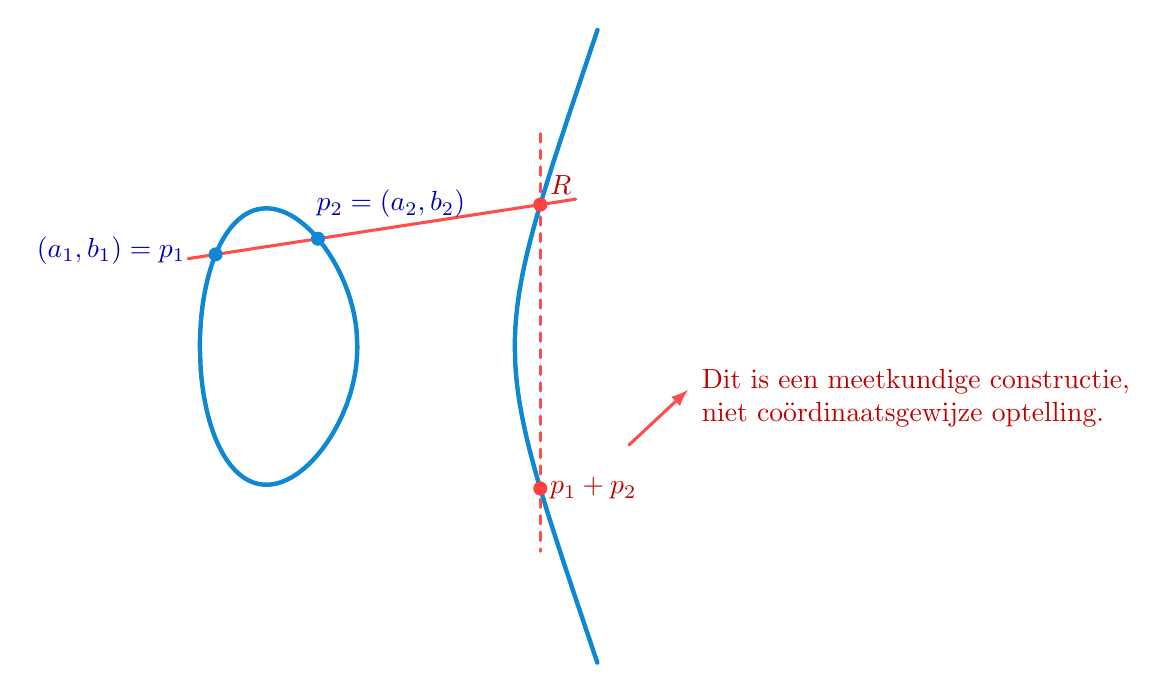
\begin{tikzpicture}[>=latex, line cap=round, line join=round]

% --- Global TikZ Styles ---
\tikzset{
    elliptic/.style={
        draw=cyan!70!blue,
        line width=1.6pt
    },
    construction/.style={
        draw=red!70,
        line width=1.1pt
    },
    constructiondashed/.style={
        draw=red!70,
        dashed,
        line width=1.1pt
    },
    bluepoint/.style={
        circle,
        fill=cyan!70!blue,
        inner sep=1.8pt
    },
    redpoint/.style={
        circle,
        fill=red!75,
        inner sep=1.8pt
    }
}

% =========================================================================
% --- Basisgeval groepswet op elliptische kromme ---
% =========================================================================

% We gebruiken dezelfde kromme als je rechterfiguur:
% y^2 = x^3 - 4x, verschoven met -1.2 in de x-richting.

\pgfmathsetmacro{\curveShift}{-1.2}

% --- Kies twee punten op de gesloten component ---
\pgfmathsetmacro{\xPone}{-1.80}
\pgfmathsetmacro{\yPone}{sqrt(abs(\xPone*\xPone*\xPone - 4*\xPone))}

\pgfmathsetmacro{\xPtwo}{-0.50}
\pgfmathsetmacro{\yPtwo}{sqrt(abs(\xPtwo*\xPtwo*\xPtwo - 4*\xPtwo))}

% --- Lijn door p_1 en p_2 ---
\pgfmathsetmacro{\msec}{(\yPtwo-\yPone)/(\xPtwo-\xPone)}
\pgfmathsetmacro{\csec}{\yPone-\msec*\xPone}

% --- Derde snijpunt R met de kromme ---
% Voor y^2 = x^3 - 4x geldt: x_R = m^2 - x_1 - x_2
\pgfmathsetmacro{\xRraw}{\msec*\msec-\xPone-\xPtwo}
\pgfmathsetmacro{\yR}{\msec*\xRraw+\csec}

% --- Verschoven x-coördinaten voor tekenen ---
\pgfmathsetmacro{\XPone}{\xPone+\curveShift}
\pgfmathsetmacro{\XPtwo}{\xPtwo+\curveShift}
\pgfmathsetmacro{\XR}{\xRraw+\curveShift}

% --- Eindpunten van de rode secantlijn ---
\pgfmathsetmacro{\lineStartX}{\XPone-0.35}
\pgfmathsetmacro{\lineStartY}{\yPone-\msec*0.35}
\pgfmathsetmacro{\lineEndX}{\XR+0.45}
\pgfmathsetmacro{\lineEndY}{\yR+\msec*0.45}

% --- Gesloten ovaalcomponent ---
\draw[elliptic]
    plot[domain=0:-2, samples=200]
        (\x + \curveShift, {sqrt(abs(\x*\x*\x - 4*\x))})
    --
    plot[domain=-2:0, samples=200]
        (\x + \curveShift, {-sqrt(abs(\x*\x*\x - 4*\x))})
    -- cycle;

% --- Rechter oneindige component ---
\draw[elliptic]
    plot[domain=3.05:2, samples=200]
        (\x + \curveShift, {sqrt(abs(\x*\x*\x - 4*\x))})
    --
    plot[domain=2:3.05, samples=200]
        (\x + \curveShift, {-sqrt(abs(\x*\x*\x - 4*\x))});

% --- Rode secantlijn door p_1 en p_2 ---
\draw[construction]
    (\lineStartX,\lineStartY) -- (\lineEndX,\lineEndY);

% --- Verticale spiegelingslijn door R ---
\draw[constructiondashed]
    (\XR,{\yR+0.9}) -- (\XR,{-\yR-0.8});

% --- Punten ---
\node[bluepoint] at (\XPone,\yPone) {};
\node[bluepoint] at (\XPtwo,\yPtwo) {};
\node[redpoint] at (\XR,\yR) {};
\node[redpoint] at (\XR,{-\yR}) {};

% --- Labels ---
\node[blue!70!black, left, xshift=-6pt] at ({\XPone-0.05},{\yPone+0.05})
    {$(a_1,b_1)=p_1$};

\node[blue!70!black, above right, yshift=4pt, xshift=-4pt] at (\XPtwo,\yPtwo)
    {$p_2=(a_2,b_2)$};

\node[red!75!black, above right] at (\XR,\yR)
    {$R$};

\node[red!75!black, right] at (\XR,{-\yR})
    {$p_1+p_2$};

% --- Opmerking rechts ---
\draw[construction, ->]
    (2.25,-1.25) -- (3.0,-0.55);
    %(3.0,-0.55) -- (2.25,-1.25);

\node[red!75!black, align=left, right] at (3.05,-0.65)
    {Dit is een meetkundige constructie,\\
     niet coördinaatsgewijze optelling.};

\end{tikzpicture}
}
\end{center}

\hl{2. Verdubbeling: $2P$}\newline
Als $P_1 = P_2 = P$, dan gebruik je niet een rechte door twee verschillende punten, maar de \hl{raaklijn} aan de kromme in $P$.
\begin{enumerate}
    \item Trek de raaklijn in $P$.
    \item Die snijdt de kromme opnieuw in een derde punt $R$.
    \item Spiegel $R$ in de $x$-as.
    \item Dat punt is
    \begin{equation*}
        2P = P + P
    \end{equation*}
\end{enumerate}

\hl{3. Speciale gevallen}\newline
\textbf{Verticaal tegenover elkaar liggende punten}\newline
Als
\begin{equation*}
    p_1 = (a,b), \qquad p_2 = (a, -b)
\end{equation*}
dan liggen ze verticaal tegenover elkaar. De rechte door $p_1$ en $p_2$ is verticaal en snijdt de kromme in het punt op oneindig. Dus
\begin{equation*}
    p_1 + p_2 = \infty
\end{equation*}

\textbf{Punten op de $x$-as}\newline
Dit is hetzelfde als een punt met zichzelf optellen, we nemen dus de raaklijn. Op de $x$-as is deze verticaal, dus het derde snijpunt is in ondeindig:
\begin{equation*}
    2P = \infty
\end{equation*}

\begin{center}
\resizebox{1.0\textwidth}{!}{%
    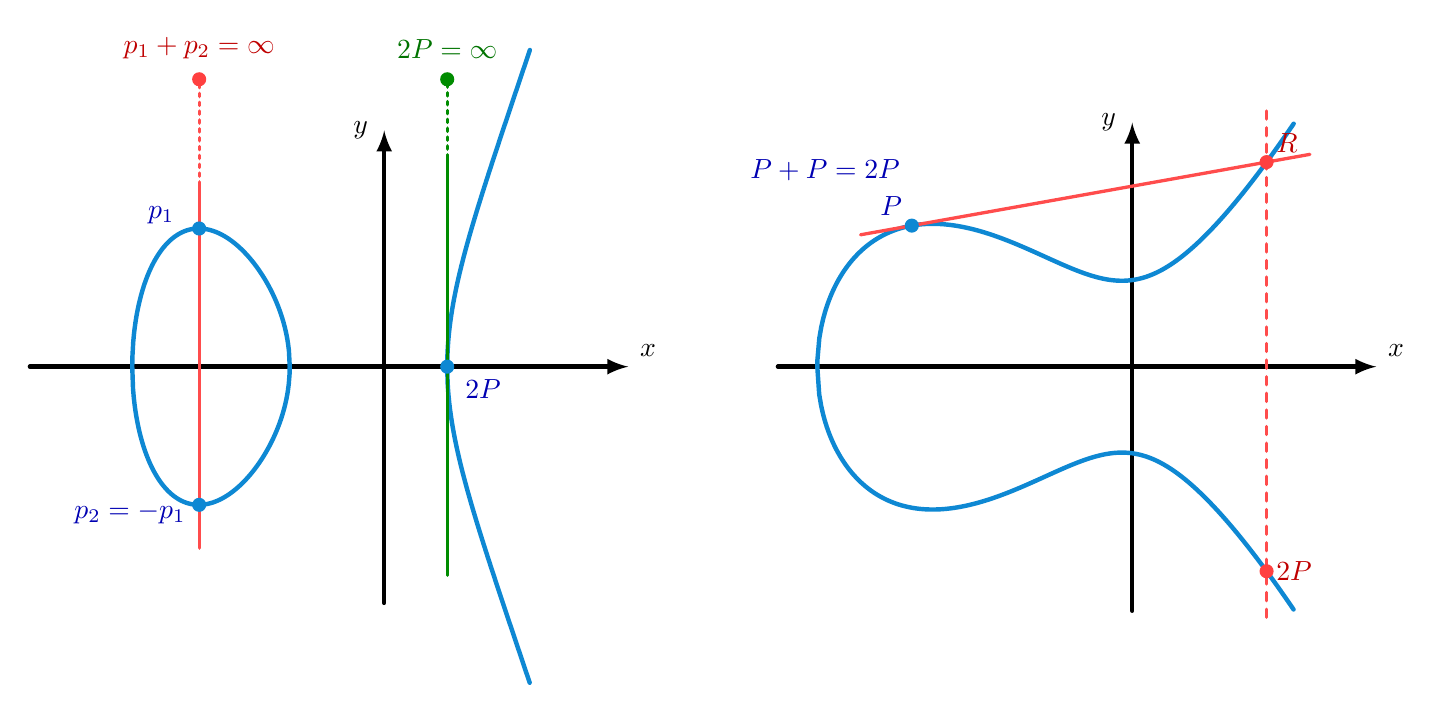
\begin{tikzpicture}[>=latex, line cap=round, line join=round]

% --- Global TikZ Styles ---
\tikzset{
    axis/.style={
        ->,
        >=latex,
        ultra thick,
        draw=black
    },
    axisline/.style={
        ultra thick,
        draw=black
    },
    elliptic/.style={
        draw=cyan!70!blue,
        line width=1.6pt
    },
    construction/.style={
        draw=red!70,
        line width=1.2pt
    },
    constructiondashed/.style={
        draw=red!70,
        dashed,
        line width=1.1pt
    },
    greenconstruction/.style={
        draw=green!55!black,
        line width=1.2pt
    },
    redpoint/.style={
        circle,
        fill=red!75,
        inner sep=1.8pt
    },
    bluepoint/.style={
        circle,
        fill=cyan!70!blue,
        inner sep=1.8pt
    },
    greenpoint/.style={
        circle,
        fill=green!55!black,
        inner sep=1.8pt
    }
}

% =========================================================================
% --- Links: p_2 = -p_1, dus p_1 + p_2 = O ---
% =========================================================================
\begin{scope}[xshift=0cm]

    \pgfmathsetmacro{\curveShift}{-1.2}

    % --- Axes ---
    \draw[axisline] (-4.5,0) -- (2.2,0);
    \draw[axis] (2.2,0) -- (3.1,0);

    \draw[axisline] (0,-3.0) -- (0,0);
    \draw[axis] (0,0) -- (0,3.0);

    \node at (3.35,0.2) {$x$};
    \node at (-0.3,3.0) {$y$};

    % --- Elliptische kromme: y^2 = x^3 - 4x, verschoven ---
    \draw[elliptic]
        plot[domain=0:-2, samples=200]
            (\x + \curveShift, {sqrt(abs(\x*\x*\x - 4*\x))})
        --
        plot[domain=-2:0, samples=200]
            (\x + \curveShift, {-sqrt(abs(\x*\x*\x - 4*\x))})
        -- cycle;

    \draw[elliptic]
        plot[domain=3.05:2, samples=200]
            (\x + \curveShift, {sqrt(abs(\x*\x*\x - 4*\x))})
        --
        plot[domain=2:3.05, samples=200]
            (\x + \curveShift, {-sqrt(abs(\x*\x*\x - 4*\x))});

    % --- Speciaal geval 1: p_2 = -p_1 ---
    \pgfmathsetmacro{\xP}{-1.15}
    \pgfmathsetmacro{\yP}{sqrt(abs(\xP*\xP*\xP - 4*\xP))}
    \pgfmathsetmacro{\XP}{\xP + \curveShift}

    % --- Verticale lijn door p_1 en p_2, verder naar oneindig ---
    \pgfmathsetmacro{\OheightRed}{3.65}

    \draw[construction]
        (\XP,{-\yP - 0.55}) -- (\XP,{\yP + 0.55});

    \draw[construction, dotted]
        (\XP,{\yP + 0.55}) -- (\XP,\OheightRed);

    \node[redpoint] at (\XP,\OheightRed) {};
    \node[red!75!black, above, yshift=4pt] at (\XP,\OheightRed) {$p_1 + p_2 = \infty$};

    % --- Blauwe punten p_1 en p_2 ---
    \node[bluepoint] at (\XP,\yP) {};
    \node[bluepoint] at (\XP,-\yP) {};

    \node[blue!70!black, left, xshift=-4pt, yshift=2pt] at ({\XP - 0.05},{\yP + 0.1}) {$p_1$};
    \node[blue!70!black, left] at ({\XP - 0.05},{-\yP - 0.1}) {$p_2=-p_1$};

    % \node[red!75!black, align=left] at (\XP,\OheightRed)
    %     {$p_1+p_2=\mathcal O$};

    % --- Speciaal geval 2: punt met verticale raaklijn ---
    \pgfmathsetmacro{\xT}{2}
    \pgfmathsetmacro{\XT}{\xT + \curveShift}

    % --- Verticale raaklijn, verder naar oneindig ---
    \pgfmathsetmacro{\OheightGreen}{3.65}

    \draw[greenconstruction]
        (\XT,-2.65) -- (\XT,2.65);

    \draw[greenconstruction, dotted]
        (\XT,2.65) -- (\XT,\OheightGreen);

    \node[greenpoint] at (\XT,\OheightGreen) {};
    \node[green!45!black, above, yshift=4pt] at (\XT,\OheightGreen) {$2P=\infty$};

    % --- Blauw punt op de x-as waar de groene lijn de kromme raakt ---
    \node[bluepoint] at (\XT,0) {};
    \node[blue!70!black, right, xshift=3pt, yshift=-8pt] at (\XT,0) {$2P$};

\end{scope}

% =========================================================================
% --- Rechts: raaklijngeval p_1 = p_2 = P ---
% =========================================================================
\begin{scope}[xshift=9.5cm]

    % We gebruiken de linkse kromme uit je oorspronkelijke figuur:
    % y^2 = x^3 + 4x^2 + x + 4,
    % met verticale compressie 0.55.

    \pgfmathsetmacro{\k}{0.55}

    % --- Axes ---
    \draw[axisline] (-4.5,0) -- (2.2,0);
    \draw[axis] (2.2,0) -- (3.1,0);

    \draw[axisline] (0,-3.1) -- (0,0);
    \draw[axis] (0,0) -- (0,3.1);

    \node at (3.35,0.2) {$x$};
    \node at (-0.3,3.1) {$y$};

    % --- Elliptische kromme ---
    \draw[elliptic]
        plot[domain=2.05:-4, samples=250]
            (\x, {\k * sqrt(abs(\x*\x*\x + 4*\x*\x + \x + 4))})
        --
        plot[domain=-4:2.05, samples=250]
            (\x, {-\k * sqrt(abs(\x*\x*\x + 4*\x*\x + \x + 4))});

    % --- Punt P en raaklijn ---
    \pgfmathsetmacro{\xP}{-2.8}
    \pgfmathsetmacro{\fP}{\xP*\xP*\xP + 4*\xP*\xP + \xP + 4}
    \pgfmathsetmacro{\yPraw}{sqrt(\fP)}
    \pgfmathsetmacro{\yP}{\k * \yPraw}

    % Helling van de raaklijn op de niet-gecomprimeerde kromme
    \pgfmathsetmacro{\mraw}{(3*\xP*\xP + 8*\xP + 1)/(2*\yPraw)}

    % Helling in de getekende, verticaal gecomprimeerde figuur
    \pgfmathsetmacro{\mdraw}{\k * \mraw}

    % Derde snijpunt R
    \pgfmathsetmacro{\xR}{\mraw*\mraw - 4 - 2*\xP}
    \pgfmathsetmacro{\yRraw}{\mraw*(\xR-\xP) + \yPraw}
    \pgfmathsetmacro{\yR}{\k * \yRraw}

    % --- Rode raaklijn ---
    \draw[construction]
        ({\xP - 0.65},{\yP - \mdraw*0.65})
        --
        ({\xR + 0.55},{\yR + \mdraw*0.55});

    % --- Spiegelingslijn door R ---
    \draw[constructiondashed]
        (\xR,{\yR + 0.65}) -- (\xR,{-\yR - 0.65});

    % --- Punten ---
    \node[bluepoint] at (\xP,\yP) {};
    \node[redpoint] at (\xR,\yR) {};
    \node[redpoint] at (\xR,-\yR) {};

    % --- Labels ---
    \node[blue!70!black, above left] at (\xP,\yP) {$P$};

    \node[red!75!black, above right] at (\xR,\yR) {$R$};

    \node[red!75!black, right] at (\xR,-\yR) {$2P$};

    \node[blue!70!black, align=left] at (-3.9,2.5)
        {$P+P=2P$};

\end{scope}

\end{tikzpicture}
}
\end{center}

\textbf{Punt op oneindig}\newline
Het punt $\infty$ behoort in principe ook tot de groep, dus moeten we het ook kunnen samenstellen. Neem bijvoorbeeld een punt $Q$. De rechte door $\infty$ en $Q$ gaat dan door een derde snijpunt $R$, dat na spiegelen met de $x$-as terug gewoon $Q$ is. Dus
\begin{equation*}
    Q + \infty = Q
\end{equation*}

\begin{center}
\resizebox{0.75\textwidth}{!}{%
    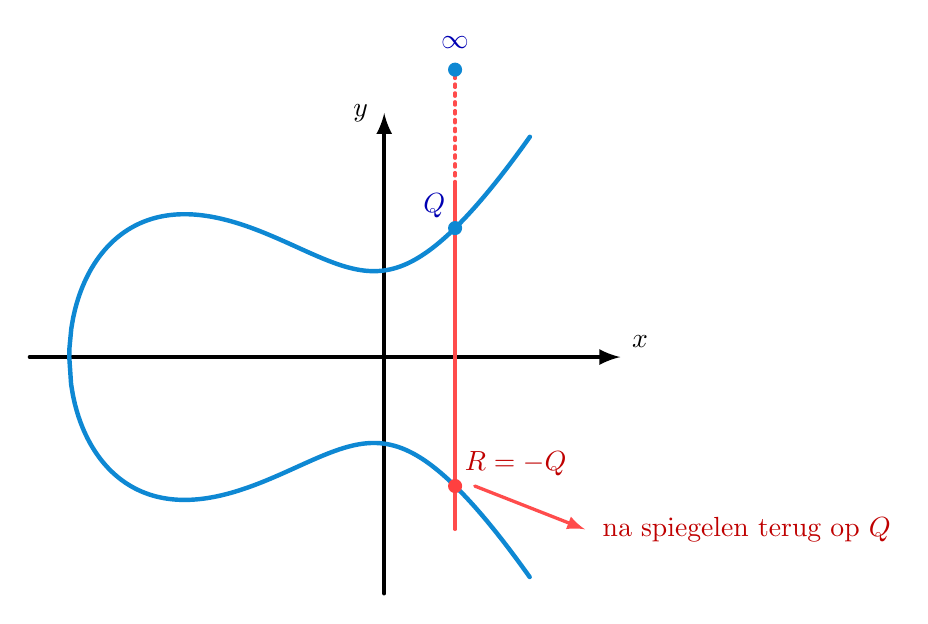
\begin{tikzpicture}[>=latex, line cap=round, line join=round]

% --- Global TikZ Styles ---
\tikzset{
    axis/.style={
        ->,
        >=latex,
        ultra thick,
        draw=black
    },
    axisline/.style={
        ultra thick,
        draw=black
    },
    elliptic/.style={
        draw=cyan!70!blue,
        line width=1.6pt
    },
    construction/.style={
        draw=red!70,
        line width=1.2pt
    },
    constructiondashed/.style={
        draw=red!70,
        dashed,
        line width=1.1pt
    },
    redpoint/.style={
        circle,
        fill=red!75,
        inner sep=1.8pt
    },
    bluepoint/.style={
        circle,
        fill=cyan!70!blue,
        inner sep=1.8pt
    }
}

% =========================================================================
% --- Neutraal element: Q + O = Q ---
% =========================================================================

% We gebruiken opnieuw de linkse kromme:
% y^2 = x^3 + 4x^2 + x + 4,
% met verticale compressie 0.55.

\pgfmathsetmacro{\k}{0.55}

% --- Axes ---
\draw[axisline] (-4.5,0) -- (2.1,0);
\draw[axis] (2.1,0) -- (3.0,0);

\draw[axisline] (0,-3.0) -- (0,0);
\draw[axis] (0,0) -- (0,3.1);

\node at (3.25,0.2) {$x$};
\node at (-0.3,3.1) {$y$};

% --- Elliptische kromme ---
\draw[elliptic]
    plot[domain=1.85:-4, samples=250]
        (\x, {\k * sqrt(abs(\x*\x*\x + 4*\x*\x + \x + 4))})
    --
    plot[domain=-4:1.85, samples=250]
        (\x, {-\k * sqrt(abs(\x*\x*\x + 4*\x*\x + \x + 4))});

% --- Punt Q en zijn inverse R = -Q ---
\pgfmathsetmacro{\xQ}{0.90}
\pgfmathsetmacro{\fQ}{\xQ*\xQ*\xQ + 4*\xQ*\xQ + \xQ + 4}
\pgfmathsetmacro{\yQ}{\k * sqrt(\fQ)}

% --- Verticale lijn door Q en O, verder naar oneindig ---
    \pgfmathsetmacro{\OheightRed}{3.65}

    \draw[construction]
        (\xQ,{-\yQ - 0.55}) -- (\xQ,{\yQ + 0.55});

    \draw[construction, dotted]
        (\xQ,{\yQ + 0.55}) -- (\xQ,\OheightRed);

    \node[bluepoint] at (\xQ,\OheightRed) {};
    \node[blue!70!black, above, yshift=4pt] at (\xQ,\OheightRed) {$\infty$};

% --- Punten op de kromme ---
\node[bluepoint] at (\xQ,\yQ) {};
\node[redpoint] at (\xQ,-\yQ) {};

% --- Labels ---
\node[blue!70!black, above left] at (\xQ,\yQ) {$Q$};
\node[red!75!black, above right] at (\xQ,-\yQ) {$R=-Q$};;

% \node[red!75!black, align=left] at (-3.9,2.45)
%     {$Q+\mathcal O=Q$};

% --- Spiegelingsaanduiding ---
\draw[construction, ->]
    ({\xQ+0.25},{-\yQ}) -- ({\xQ+1.65},{-\yQ-0.55});

\node[red!75!black, align=left, right] at ({\xQ+1.75},{-\yQ-0.55})
    {na spiegelen terug op $Q$};

\end{tikzpicture}
}
\end{center}

\begin{nicetheorem}*
    \nextpart[]*
    Met deze optelling is
    \begin{equation*}
        \langle E(K), + \rangle
    \end{equation*}
    een \hl[red!75!black]{commutatieve groep}.
\end{nicetheorem}
Bewijs niet kennen.

Uit de bovenstaande voorbeelden kunnen we ook eigenschappen afleiden.

Uit de samenstelling met een punt op oneindig weet je $Q + \infty = Q$. M.a.w. $\infty$ is het neutraal element.

\begin{niceproperty}*[Neutraal element]
    \nextpart[]*
    In de commutatieve groep $\langle E(K), + \rangle$ is $\infty$ het \hl[RoyalPurple!75!black]{neutrale element}.
\end{niceproperty}

Ook weten we dat, als we twee verticaal tegenover elkaar liggende punten $p_1 = (a,b)$ en $p_2 = (a, -b)$ nemen, dat $p_1 + p_2 = \infty = 0$ (herinner neutrale element). M.a.w. $p_2$ is de inverse van $p_1$.

\begin{niceproperty}*[Invers element]
    \nextpart[]*
    In de commutatieve groep $\langle E(K), + \rangle$ is het \hl[RoyalPurple!75!black]{inverse element} voor een punt
    \begin{equation*}
        -(a,b) = (a, -b)
    \end{equation*}
\end{niceproperty}

\subsubsection{Expliciete formules voor de groepswet}

\begin{center}
\resizebox{0.65\textwidth}{!}{%
    \input{figures/L8/expliciete_formules.tex}
}
\end{center}

Voor berekeningen over eindige velden hebben we algebraïsche formules nodig. Neem
\begin{equation*}
    P_1 = (a_1, b_1) \qquad \text{en} \qquad P_2 = (a_2, b_2)
\end{equation*}
en schrijf
\begin{equation*}
    P_1 + P_2 = (a_3, b_3)
\end{equation*}
De kromme is
\begin{equation*}
    E : y^2 = x^3 + Ax + B
\end{equation*}

\SimpleHeading{Richtingscoëfficiënt}

Als $P_1 \neq P_2$, dan is de richtingscoëfficiënt van de rechte door beide punten gewoon
\begin{equation*}
    \lambda = \frac{\Delta y}{\Delta x} = \frac{b_2 - b_1}{a_2 - a_1}
\end{equation*}
Als $P_1 = P_2$, dan gebruiken we de raaklijn aan de kromme door dit punt. De richtingscoëfficiënt van een raaklijn is de afgeleide $dx/dy$.
\begin{equation*}
    \begin{aligned}
        \frac{d}{dx}(y^2) &= \frac{d}{dx}(x^3 + Ax + B) \\
        2y \cdot \frac{dy}{dx} &= 3x^2 + A \\
        \frac{dy}{dx} &= \frac{3x^2 + A}{2y}
    \end{aligned}
\end{equation*}
Invullen in het punt $(a_1, b_1)$ geeft dan direct de gewenste richtingscoëfficiënt:
\begin{equation*}
    \lambda = \frac{3a_1^2 + A}{2b_1}
\end{equation*}

\SimpleHeading{Coördinaten van de som}

We hebben nu de recht $y = \lambda(x-a_1) + b_1$ met richtingscoëfficiënt $\lambda$ die door $P_1$ en $P_2$ loopt. 

\hl{Stap A: we zoeken het snijpunt van de rechte met de kromme} \newline
We lossen het stelsel op:
\begin{enumerate}
    \item Kromme: $y^2 = x^3 + Ax + B$
    \item rechte: $y = \lambda(x-a_1) + b_1$
\end{enumerate}
(1) in (2) substitueren geeft:
\begin{equation*}
    \left(y = \lambda(x-a_1) + b_1\right)^2 = x^3 + Ax + B
\end{equation*}
Dit uitwerken resulteert in een derdegraadsvergelijking in $x$ van de vorm:
\begin{equation*}
    x^3 - \lambda^2 x^2 + \cdots = 0 
\end{equation*}

\hl{Stap B: formule $a_3$ afleiden} \newline
Volgens de \hl{Regels van Viète} is de som van de drie wortels $x_1$, $x_2$, $x_3$ van een veelterm $x^3 + cx^2 + dx + e = 0$ gelijk aan $-c$.

In onze vergelijking is de coëfficiënt voor $x^2$ gelijk aan $-\lambda^2$. Dus geldt:
\begin{equation*}
    x_1 + x_2 + x_3 = \lambda^2
\end{equation*}
We weten al dat $x_1 = a_1$ en $x_2 = a_2$ al snijpunten zijn. Het derde snijpunt heeft $x$-coördinaat $a'_3$:
\begin{equation*}
    a_1 + a_2 + a'_3 = \lambda^2 \implies a'_3 = \lambda^2 - a_1 - a_2
\end{equation*}
Herinner dat de optelling volgens de groepswet zegt dat we het derde snijpunt moeten spiegelen over de $x$-as, de $x$-coördinaat verandert dus niet. 

Voor ons sompunt $P_3 = (a_3, b_3)$ geldt dus gewoon:
\begin{equationbox}*[NavyBlue][SkyBlue!10]
    a_3 = \lambda^2 - a_1 - a_2
\end{equationbox}

\hl{Stap C: formule $b_3$ afleiden} \newline
Het derde (onbekende) snijpunt op de lijn $(a_3, b'_3)$ heeft een $y$-coördinaat $b'_3$ die voldoet aan de vergelijking:
\begin{equation*}
    b'_3 = \lambda (a_3 - a_1) + b_1
\end{equation*}
Vergeet niet dat ons uiteindelijke punt $P_3 = (a_3, b_3)$ de \hl{gespiegelde versie} is van dit snijpunt over de $x$-as ($b_3 = -b'_3$):
\begin{equation*}
    b_3 = -\left(\lambda(a_3 - a_1) + b_1\right) = -b_1 - \lambda (a_3 - a_1)
\end{equation*}
Dit uitwerken geeft:
\begin{equationbox}*[NavyBlue][SkyBlue!10]
    b_3 = \lambda (a_1 - a_3) - b_1
\end{equationbox}

\subsubsection{Elliptic Curve Diffie-Hellman}

Voor cryptografie kiest men:
\begin{itemize}
    \item een elliptische kromme $E$ over een eindig veld $\mathbb{F}_q$.
    \item een punt $P \in E(\mathbb{F}_q)$ dat een cyclische deelgroep van grote priemorde $l$ voortbrengt. $\langle P \rangle = \{1P, 2P, 3P, \dots, (l-1)P, lP=\infty\}$
\end{itemize}
De \textcolor{Emerald}{publieke parameters} zijn dan: $E, \mathbb{F}_q, P$ en $l$.

\SimpleHeading{Protocol}

\textbf{1.} Alice kies \textcolor{WildStrawberry}{geheim}
\begin{equation*}
    \textcolor{WildStrawberry}{a} \in \{0, 1, \dots, l-1\}
\end{equation*}
en stuurt $\textcolor{WildStrawberry}{a}P$ naar Bob.

\textbf{2.} Bob kiest \textcolor{BurntOrange}{geheim}
\begin{equation*}
    \textcolor{BurntOrange}{b} \in \{0, 1, \dots, l-1\}
\end{equation*}
en stuurt $\textcolor{WildStrawberry}{b}P$ naar Alice.

\textbf{3.} Alice berekent: $\textcolor{WildStrawberry}{a}(\textcolor{BurntOrange}{b}P) = \textcolor{WildStrawberry}{a}\textcolor{BurntOrange}{b}P$

\textbf{4.} Bob berekent: $\textcolor{BurntOrange}{b}(\textcolor{WildStrawberry}{a}P) = \textcolor{WildStrawberry}{a}\textcolor{BurntOrange}{b}P$

$\rightwhitearrow$ Beiden komen dus uit op hetzelfde punt $abP$. Dat punt wordt daarna omgezet naar bijvoorbeeld een AES-sleutel.

\begin{center}
\resizebox{0.82\textwidth}{!}{%
    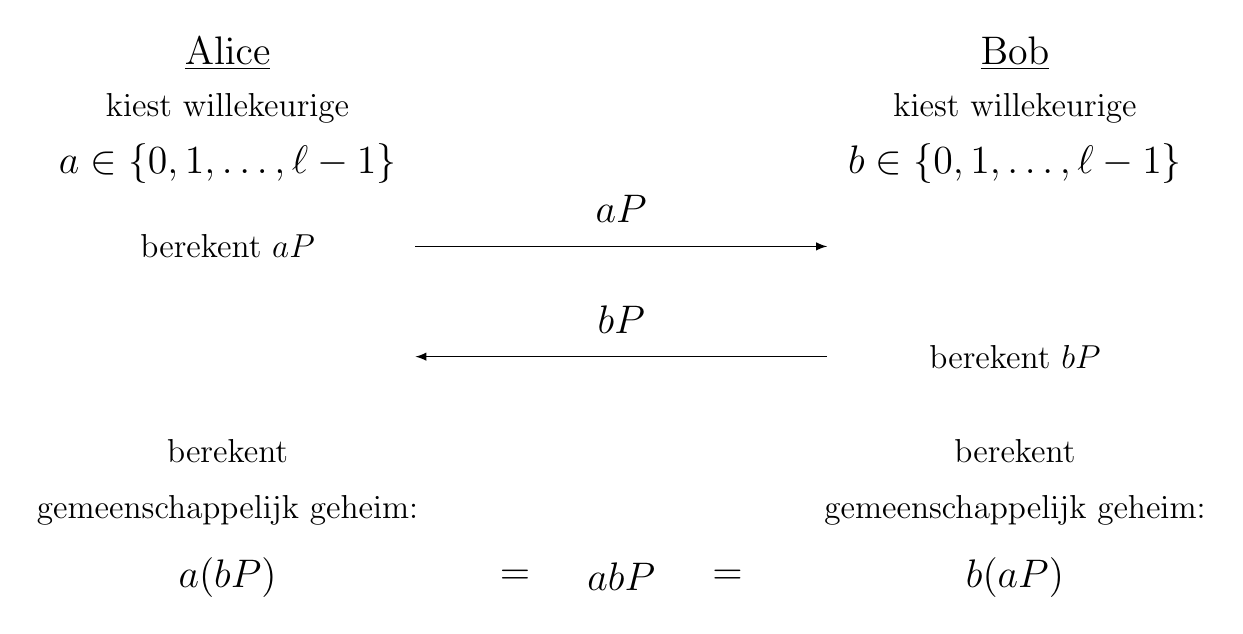
\begin{tikzpicture}[
    >=latex,
    textline/.style={
        font=\large,
        align=center
    },
    person/.style={
        font=\Large
    },
    formula/.style={
        font=\Large
    },
    message/.style={
        ->,
        thin,
        shorten >=1pt,
        shorten <=1pt
    }
]

% Horizontal positions of Alice and Bob
\def\AliceX{0}
\def\BobX{10}

% ==================================================
% Alice
% ==================================================

\node[person] at (\AliceX,4.8)
    {\underline{Alice}};

\node[textline] at (\AliceX,4.1)
    {kiest willekeurige};

\node[formula] at (\AliceX,3.4)
    {$a \in \{0,1,\ldots,\ell-1\}$};

\node[textline] at (\AliceX,2.35)
    {berekent $aP$};

% ==================================================
% Bob
% ==================================================

\node[person] at (\BobX,4.8)
    {\underline{Bob}};

\node[textline] at (\BobX,4.1)
    {kiest willekeurige};

\node[formula] at (\BobX,3.4)
    {$b \in \{0,1,\ldots,\ell-1\}$};

\node[textline] at (\BobX,0.95)
    {berekent $bP$};

% ==================================================
% Exchanged values
% ==================================================

% Alice sends aP to Bob
\draw[message]
    (2.35,2.35)
    --
    node[above=5pt, font=\Large] {$aP$}
    (7.65,2.35);

% Bob sends bP to Alice
\draw[message]
    (7.65,0.95)
    --
    node[above=5pt, font=\Large] {$bP$}
    (2.35,0.95);

% ==================================================
% Shared secret calculations
% ==================================================

% Alice's calculation
\node[textline] at (\AliceX,-0.25)
    {berekent};

\node[textline] at (\AliceX,-1.0)
    {gemeenschappelijk geheim:};

\node[formula] at (\AliceX,-1.85)
    {$a(bP)$};

% Bob's calculation
\node[textline] at (\BobX,-0.25)
    {berekent};

\node[textline] at (\BobX,-1.0)
    {gemeenschappelijk geheim:};

\node[formula] at (\BobX,-1.85)
    {$b(aP)$};

% Equality in the middle
\node[formula] at (3.65,-1.85) {$=$};
\node[formula] at (5.00,-1.85) {$abP$};
\node[formula] at (6.35,-1.85) {$=$};

\end{tikzpicture}
}
\end{center}

\SimpleHeading{Veiligheidsaanname}

Een aanvaller ziet $P$, $aP$ en $bP$, maar zou $abP$ moeten vinden. De evident manier is om uit $aP$ de scalar $a$ te halen. Maar dat is precies het DLP op elliptische krommen:
\begin{equation*}
    P, aP \longrightarrow a
\end{equation*}
Dit klinkt misschien vreemd, waarom is uit $aP$ proberen $a$ te berekenen een DLP?
\begin{enumerate}
    \item Het "machtsverheffen" (forward operation):\newline
    Gegeven een punt $P$ en een geheim getal $a$, bereken het punt $Q = aP$. Dit kan supersnel met het square-and-multipl of double-and-add algoritme (zie \Cref{sec:l8_aP-berekenen}).

    \item Het "Discrete Logaritme" (reverse operation):\newline
    Gegeven een startpunt $P$ en een eindpunt $Q = aP$, vind het geheime getal $a$.
    \begin{equation*}
        \text{vind } a = \log_P(Q)
    \end{equation*}
    Omdat de bewerking $aP$ kriskras over de kromme spring, is er geen gemakkelijke formule om $a$ direct uit $aP$ en $P$ te berekenen. Een aanvaller zou in het ergste geval alle mogelijkheden voor $a$ moeten proberen.
\end{enumerate}

\subsubsection{Scalarvermenigvuldiging: \texorpdfstring{$aP$}{aP} berekenen}\label{sec:l8_aP-berekenen}

Naïef $aP$ berekenen als
\begin{equation*}
    P + P + \cdots + P
\end{equation*}
met $a$ termen is onmogelijk als $a$ ongeveer 256 bits lang is.

Daarom gebruikt men \hl{verdubbelen-en-optellen}. Dit is de additieve versie van \hl{square-and-multiply}.

Schrijf $a$ binair:
\begin{equation*}
    a = a_0 + a_1 2 + a_2 2^2 + \cdots a_r 2^r
\end{equation*}
met $a_i \in \{0,1\}$.

Bereken eerst door herhaald verdubbelen:
\begin{equation*}
    P, 2P, 2^2P, 2^3P, \dots, 2^rP
\end{equation*}
Dan is
\begin{equation*}
    aP = \sum_{i:a_i = 1}2^iP
\end{equation*}
$i:a_i = 1$ wil gewoon zeggen "neem de som over alle indexen $i$ waarvoor de bit $a_i$ gelijk is aan 1".

\textbf{\underbar{Voorbeeld:}} Stel we willen $aP$ berekenen voor $a=13$.
\begin{enumerate}
    \item Zet $a=13$ om naar binair: $13 = 1101_2$\newline
    Dit betekent gewoon:
    \begin{itemize}
        \item $a_0 = 1$
        \item $a_1 = 0$
        \item $a_2 = 1$
        \item $a_3 = 1$
    \end{itemize}
    \item Bereken de verdubbelingen $(P, 2P, 2^2P, 2^3P)$. \newline
    Dit kost maar 3 verdubbelingen $(P\to2P\to4P\to8P)$.
    \item Pas de formule toe. We kijken welke bitjes op 1 staan ($i=0,2,3$) en tellen alleen die punten op:
    \begin{equation*}
        13P = (1 \cdot 2^3P) + (1 \cdot 2^2P) + (0 \cdot 2^1P) + (1 \cdot 2^0P)
    \end{equation*}
    \begin{equation*}
        13P = 8P + 4P + P
    \end{equation*}
    $\rightwhitearrow$ Dus voor $13P$ te berekenen heb je maar slechts 3 verdubbelingen en 2 optellingen nodig. Trek je dit door naar een 256-bit getal, dan vraagt dit algoritme gemiddeld maar 256 verdubbelingen en 128 optellingen. Verglijk dit met de naïve $2^{256}$ optellingen!
\end{enumerate}

\section*{Codetheorie}

\tocdecorline{Hoofdtuk 5 -- Codetheorie}

\subsection{Motivatie -- Codetheorie}

De setting lijkt op cryptografie: een boodschap wordt over een onbetrouwbaar kanaal verstuurd. Maar "onbetrouwbaar" betekent hier iets anders.
\begin{itemize}
    \item In cryptografie: iemand kan meeluisteren of berichten manipuleren.
    \item In codetheorie: er treedt \hl{ruis} op, waardoor sommige symbolen of bits veranderen
\end{itemize}

\begin{center}
\resizebox{0.60\textwidth}{!}{%
    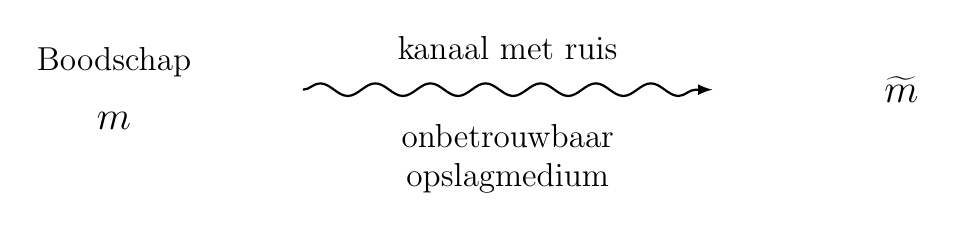
\begin{tikzpicture}[
    >=latex,
    textline/.style={
        font=\large,
        align=center
    },
    formula/.style={
        font=\Large
    },
    noisy channel/.style={
        ->,
        thick,
        decorate,
        decoration={
            snake,
            amplitude=0.8mm,
            segment length=7mm,
            post length=2mm
        }
    }
]

% Horizontal positions
\def\MessageX{0}
\def\ChannelStart{2.4}
\def\ChannelEnd{7.6}
\def\OutputX{10}

% Original message
\node[textline] at (\MessageX,0.75)
    {Boodschap};

\node[formula] at (\MessageX,0)
    {$m$};

% Noisy channel
\draw[noisy channel]
    (\ChannelStart,0.4)
    --
    node[
        above=7pt,
        textline
    ]
    {kanaal met ruis}
    node[
        below=9pt,
        textline
    ]
    {onbetrouwbaar\\opslagmedium}
    (\ChannelEnd,0.4);

% Possibly corrupted message
\node[formula] at (\OutputX,0.4)
    {$\widetilde{m}$};

\end{tikzpicture}
}
\end{center}

Voorbeelden:
\begin{itemize}
    \item CD's, DVD's en opslagmedia;
    \item harde schijven;
    \item satellietcommunicatie;
    \item communicatie met ruimtesondes zoals Voyager;
    \item QR-codes;
    \item digitale netwerken.
\end{itemize}
Het doel is fouten te \hl{detecteren} en indien mogelijk te \hl{corrigeren}. Het basisidee is dus:
\begin{center}
    Voeg \hl{redundantie} toe aan de boodschap.
\end{center}

\subsubsection{Voorbeeld: pariteitsbit}

Neem een binaire boodschap
\begin{equation*}
    m = (m_1, \dots, m_{n-1}) \in \mathbb{F}_2^{n-1}
\end{equation*}
Dit is de oorspronkelijke boodschap, een rijtje van $n-1$ nullen en enen. Je voegt hier nu één extra bit acteraan aan toe: $p = m_1 + m_2 + \cdots + m_{n-1}$. Het totale codewoord $c$ heeft dan lengte $n$:
\begin{equation*}
    c = (m_1, m_2, \dots, m_{n-1}, \underbrace{m_1 + \cdots + m_{n-1}}_{\text{pariteitsbit}})
\end{equation*}
\hl{Waarom maakt dit het totaal aantal enen even?}\newline
in $\mathbb{F}_2$ geldt $1+1=0$ (optellen is XOR).
\begin{itemize}
    \item Als er een EVEN aantal enen in $m$ zit:\newline
    De som $m_1 + \cdots + m_{n-1} = 0$. De pariteitsbit wordt 0. Het totaal aantal even blijft \textbf{even}.
    \item Als er een ONEVEN aantal enen in $m$ zit:\newline
    De som $m_1 + \cdots + m_{n-1} = 1$. De pariteitsbit wordt 1. Met die extra 1 erbij wordt het totale aantal enen \textbf{even}.
\end{itemize}
\textbf{De regel:} Elk geldig codewoord $c$ bevat altijd een \textbf{even aantal enen!}

\hl{Waarom doet dit foutdetectie?}\newline
Stel dat de ontvanger een bericht binnenkrijgt. Hij telt het aantal enen.

Als er onderweg precies 1 bit flipt ($0\to1$ of $1\to0$), dan verandert de pariteit van even naar \textbf{oneven}.

De ontvanger telt een oneven aantal enen en weet meteen: "Er is onderweg iets misgegaan!"

\hl{Beperkingen}
\begin{enumerate}
    \item Geen fout\hl{correctie}. Kan detecteren, niet herstellen.
    \item Onzichtbaar voor dubbele fouten.
\end{enumerate}


\subsubsection{Algemene setting van codes}

\begin{center}
\resizebox{1.00\textwidth}{!}{%
    \begin{tikzpicture}[
    >=latex,
    formula/.style={
        font=\Large
    },
    textline/.style={
        font=\large,
        align=center
    },
    message/.style={
        ->,
        thin,
        shorten >=1pt,
        shorten <=1pt
    },
    noisy channel/.style={
        ->,
        thin,
        decorate,
        decoration={
            snake,
            amplitude=0.8mm,
            segment length=7mm,
            post length=2mm
        }
    }
]

% ==================================================
% Message and encoding
% ==================================================

\node[formula] (message) at (0,0)
    {$m$};

\node[formula] (codeword) at (3,0)
    {$c=f(m)$};

\draw[message]
    (message.east)
    --
    (codeword.west);

% ==================================================
% Noisy channel
% ==================================================

\node[formula] (received) at (8,0)
    {$\widetilde{c}$};

\draw[noisy channel]
    (codeword.east)
    --
    (received.west);

% ==================================================
% Error correction
% ==================================================

\node[formula] (corrected) at (12.7,0)
    {$\overline{c}\in C$};

\draw[message]
    (received.east)
    --
    node[
        above=5pt,
        textline
    ]
    {fouten-\\verbetering}
    (corrected.west);

% ==================================================
% Decoding
% ==================================================

\node[formula] (decoded) at (17,0)
    {$\overline{m}$};

\draw[message]
    (corrected.east)
    --
    node[
        above=6pt,
        formula
    ]
    {$f^{-1}$}
    (decoded.west);

% ==================================================
% Desired result
% ==================================================

\node[
    textline,
    anchor=west
] (hopefully) at (18.3,-1.1)
    {hopelijk $m$};

\draw[message]
    (decoded.south)
    |-
    (hopefully.west);

\end{tikzpicture}
}
\end{center}

\subsection{lineaire codes}

\subsubsection{Generatormatrix}

\subsubsection{Systematische codes}

\subsubsection{Pariteitscontrole als lineaire code}

\subsubsection{Pariteitscontrolematrix bij systematische codes}

\subsection{Foutdetectie via pariteitscontrole}

\subsubsection{Nearest-neighbour decoding}

\subsubsection{Hamming-gewicht en Hamming-afstand}

\subsubsection{Geometrisch idee achter foutcorrectie}

\subsection{Recap -- Kernpunten van deze les}

\subsection{Samenvattende oefeningen}

\begin{niceexercise}*\label{ex:l8_groep-DLP-easy}
    \nextpart[]*
    Toon aan dat in een cryptografisch systeem dat is gebaseerd op de groep $\langle \mathbb{F}_p, \textcolor{Red}{+}\rangle$ onveilig is, want het DLP is hier gemakkelijk.
\end{niceexercise}

Normaal gesproken kijken we naar de multiplicatieve groep $\langle \mathbb{F}_p^\times, \cdot \rangle$. Het DLP is dan als volgt gedefinieerd:
\begin{itemize}
    \item Gegegven een basis $g$ en een element $y$,
    \item[$\to$] Zoek de geheime $x$ waarvoor geldt: $g^x \equiv y \pmod p$
\end{itemize}
We hebben eerder al gezien dat dit moeilijk is. Wat verandert er nu in de additieve groep $\langle \mathbb{F}_p, + \rangle$?

In de additieve groep $\mathbb{F}_p$ is de groepsbewerking niet vermenigvuldigen, maar optellen. Wanneer we in een additieve groep een element $g$ "machtsverheffen" tot de macht $x$, betekent dat niet $g \cdot g \cdot \dots \dot g$, maar dat we $g$ $x$ keer bij zichzelf optellen:
\begin{equation*}
    \underbrace{g + g + \cdots + g}_{x \text{ keer}} \equiv y \mod p
\end{equation*}
Maar $x$ keer $g$ bij zichzelf optellen is natuurlijk gewoone vermenigvuldiging:
\begin{equation*}
    x \cdot g \equiv y \pmod p
\end{equation*}
Waarom is het DLP hier nu dan triviaal? We hebben het DLP in $\langle \mathbb{F}_p, + \rangle$ net herleid tot de vergelijking $x \cdot g \equiv y \pmod p$. I.p.v. dat we een moeilijke exponent $x$ moeten zoeken, zoeken we nu gewoon de factor $x$. En hoe los je een gewone lineaire vergelijking op modulo $p$?
Door te delen door $g$! Dat is dus gewoon vermenigvuldigen met de modulaire inverse van $g$:
\begin{equation*}
    x \equiv y \cdot g^{-1} \pmod p
\end{equation*}
Het uitgebreide algoritme van Euclides kan dit extreem snel berekenen!